\documentclass[10pt]{article}\usepackage[]{graphicx}\usepackage[]{xcolor}
%% maxwidth is the original width if it is less than linewidth
%% otherwise use linewidth (to make sure the graphics do not exceed the margin)
\makeatletter
\def\maxwidth{ %
  \ifdim\Gin@nat@width>\linewidth
    \linewidth
  \else
    \Gin@nat@width
  \fi
}
\makeatother

\definecolor{fgcolor}{rgb}{0.345, 0.345, 0.345}
\newcommand{\hlnum}[1]{\textcolor[rgb]{0.686,0.059,0.569}{#1} }%
\newcommand{\hlstr}[1]{\textcolor[rgb]{0.192,0.494,0.8}{#1} }%
\newcommand{\hlcom}[1]{\textcolor[rgb]{0.678,0.584,0.686}{\textit{#1} } }%
\newcommand{\hlopt}[1]{\textcolor[rgb]{0,0,0}{#1} }%
\newcommand{\hlstd}[1]{\textcolor[rgb]{0.345,0.345,0.345}{#1} }%
\newcommand{\hlkwa}[1]{\textcolor[rgb]{0.161,0.373,0.58}{\textbf{#1} } }%
\newcommand{\hlkwb}[1]{\textcolor[rgb]{0.69,0.353,0.396}{#1} }%
\newcommand{\hlkwc}[1]{\textcolor[rgb]{0.333,0.667,0.333}{#1} }%
\newcommand{\hlkwd}[1]{\textcolor[rgb]{0.737,0.353,0.396}{\textbf{#1} } }%

\usepackage{framed}
\makeatletter
\newenvironment{kframe}{%
 \def\at@end@of@kframe{}%
 \ifinner\ifhmode%
  \def\at@end@of@kframe{\end{minipage} }%
  \begin{minipage}{\columnwidth}%
 \fi\fi%
 \def\FrameCommand##1{\hskip\@totalleftmargin \hskip-\fboxsep
 \colorbox{shadecolor}{##1}\hskip-\fboxsep
     % There is no \\@totalrightmargin, so:
     \hskip-\linewidth \hskip-\@totalleftmargin \hskip\columnwidth}%
 \MakeFramed {\advance\hsize-\width
   \@totalleftmargin\z@ \linewidth\hsize
   \@setminipage} }%
 {\par\unskip\endMakeFramed%
 \at@end@of@kframe}
\makeatother

\definecolor{shadecolor}{rgb}{.97, .97, .97}
\definecolor{messagecolor}{rgb}{0, 0, 0}
\definecolor{warningcolor}{rgb}{1, 0, 1}
\definecolor{errorcolor}{rgb}{1, 0, 0}
\newenvironment{knitrout}{}{} % an empty environment to be redefined in TeX

\usepackage{alltt}

%%%%%%%%%%%%%%%%%%%%%%%%%%%%%%%%%%%%%%%%%%%%%%%%%%%%%%%%%%%%%%%%%%%%%%%%%%%%%%%%
% LaTeX Imports
%%%%%%%%%%%%%%%%%%%%%%%%%%%%%%%%%%%%%%%%%%%%%%%%%%%%%%%%%%%%%%%%%%%%%%%%%%%%%%%%
\usepackage{amsfonts}                                                   % Math fonts
\usepackage{amsmath}                                                    % Math formatting
\usepackage{amssymb}                                                    % Math formatting
\usepackage{amsthm}                                                     % Math Theorems
\usepackage{arydshln}                                                   % Dashed hlines
\usepackage{attachfile}                                                 % AttachFiles
\usepackage{cancel}                                                     % Cancelled math
\usepackage{caption}                                                    % Figure captioning
\usepackage{color}                                                      % Nice Colors
\input{./lib/dragon.inp}                                                % Tikz dragon curve
\usepackage[ampersand]{easylist}                                        % Easy lists
\usepackage{fancyhdr}                                                   % Fancy Header
\usepackage[T1]{fontenc}                                                % Specific font-encoding
%\usepackage[margin=1in, marginparwidth=2cm, marginparsep=2cm]{geometry} % Margins
\usepackage{graphicx}                                                   % Include images
\usepackage{hyperref}                                                   % Referencing
\usepackage[none]{hyphenat}                                             % Don't allow hyphenation
\usepackage{lipsum}                                                     % Lorem Ipsum Dummy Text
\usepackage{listings}                                                   % Code display
\usepackage{marginnote}                                                 % Notes in the margin
\usepackage{microtype}                                                  % Niceness
\usepackage{lib/minted}                                                 % Code display
\usepackage{multirow}                                                   % Multirow tables
\usepackage{pdfpages}                                                   % Include pdfs
\usepackage{pgfplots}                                                   % Create Pictures
\usepackage{rotating}                                                   % Figure rotation
\usepackage{setspace}                                                   % Allow double spacing
\usepackage{subcaption}                                                 % Figure captioning
\usepackage{tikz}                                                       % Create Pictures
\usepackage{tocloft}                                                    % List of Equations
%%%%%%%%%%%%%%%%%%%%%%%%%%%%%%%%%%%%%%%%%%%%%%%%%%%%%%%%%%%%%%%%%%%%%%%%%%%%%%%%
% Package Setup
%%%%%%%%%%%%%%%%%%%%%%%%%%%%%%%%%%%%%%%%%%%%%%%%%%%%%%%%%%%%%%%%%%%%%%%%%%%%%%%%
\hypersetup{%                                                           % Setup linking
    colorlinks=true,
    linkcolor=black,
    citecolor=black,
    filecolor=black,
    urlcolor=black,
}
\RequirePackage[l2tabu, orthodox]{nag}                                  % Nag about bad syntax
\renewcommand*\thesection{\arabic{section} }                             % Reset numbering
\renewcommand{\theFancyVerbLine}{ {\arabic{FancyVerbLine} } }              % Needed for code display
\renewcommand{\footrulewidth}{0.4pt}                                    % Footer hline
\setcounter{secnumdepth}{3}                                             % Include subsubsections in numbering
\setcounter{tocdepth}{3}                                                % Include subsubsections in toc
%%%%%%%%%%%%%%%%%%%%%%%%%%%%%%%%%%%%%%%%%%%%%%%%%%%%%%%%%%%%%%%%%%%%%%%%%%%%%%%%
% Custom commands
%%%%%%%%%%%%%%%%%%%%%%%%%%%%%%%%%%%%%%%%%%%%%%%%%%%%%%%%%%%%%%%%%%%%%%%%%%%%%%%%
\newcommand{\nvec}[1]{\left\langle #1 \right\rangle}                    %  Easy to use vector
\newcommand{\ma}[0]{\mathbf{A} }                                         %  Easy to use vector
\newcommand{\mb}[0]{\mathbf{B} }                                         %  Easy to use vector
\newcommand{\abs}[1]{\left\lvert #1 \right\rvert}                       %  Easy to use abs
\newcommand{\pren}[1]{\left( #1 \right)}                                %  Big parens
\let\oldvec\vec
\renewcommand{\vec}[1]{\oldvec{\mathbf{#1} } }                            %  Vector Styling
\newtheorem{thm}{Theorem}                                               %  Define the theorem name
\newtheorem{definition}{Definition}                                     %  Define the definition name
\definecolor{bg}{rgb}{0.95,0.95,0.95}
\newcommand{\java}[4]{\vspace{10pt}\inputminted[firstline=#2,
                                 lastline=#3,
                                 firstnumber=#2,
                                 gobble=#4,
                                 frame=single,
                                 label=#1,
                                 bgcolor=bg,
                                 linenos]{java}{#1} }
\newcommand{\python}[4]{\vspace{10pt}\inputminted[firstline=#2,
                                 lastline=#3,
                                 firstnumber=#2,
                                 gobble=#4,
                                 frame=single,
                                 label=#1,
                                 bgcolor=bg,
                                 linenos]{python}{#1} }
\newcommand{\js}[4]{\vspace{10pt}\inputminted[firstline=#2,
                                 lastline=#3,
                                 firstnumber=#2,
                                 gobble=#4,
                                 frame=single,
                                 label=#1,
                                 bgcolor=bg,
                                 linenos]{js}{#1} }
%%%%%%%%%%%%%%%%%%%%%%%%%%%%%%%%%%%%%%%%%%%%%%%%%%%%%%%%%%%%%%%%%%%%%%%%%%%%%%%%
% Beginning of document items - headers, title, toc, etc...
%%%%%%%%%%%%%%%%%%%%%%%%%%%%%%%%%%%%%%%%%%%%%%%%%%%%%%%%%%%%%%%%%%%%%%%%%%%%%%%%
\pagestyle{fancy}                                                       %  Establishes that the headers will be defined
\fancyhead[LE,LO]{Computer Systems Notes}                                  %  Adds header to left
\fancyhead[RE,RO]{Zoe Farmer}                                       %  Adds header to right
\cfoot{ \thepage }
\lfoot{CSCI 2400}
\rfoot{Han}
\title{Computer Systems Notes}
\author{Zoe Farmer}

%%%%%%%%%%%%%%%%%%%%%%%%%%%%%%%%%%%%%%%%%%%%%%%%%%%%%%%%%%%%%%%%%%%%%%%%%%%%%%%%
% Beginning of document items - headers, title, toc, etc...
%%%%%%%%%%%%%%%%%%%%%%%%%%%%%%%%%%%%%%%%%%%%%%%%%%%%%%%%%%%%%%%%%%%%%%%%%%%%%%%%
\pagestyle{fancy}                                                       %  Establishes that the headers will be defined
\fancyhead[LE,LO]{Homework 9}                                  %  Adds header to left
\fancyhead[RE,RO]{Zoe Farmer}                                       %  Adds header to right
\cfoot{\mlptikz[size=0.25in, text=on, textposx=0, textposy=0, textvalue=\thepage, textscale=0.75in]{applejack} }
\lfoot{APPM 3570}
\rfoot{Kleiber}
\title{Homework 9}
\date{Kleiber}
\author{Zoe Farmer - 101446930}
%%%%%%%%%%%%%%%%%%%%%%%%%%%%%%%%%%%%%%%%%%%%%%%%%%%%%%%%%%%%%%%%%%%%%%%%%%%%%%%%
% Beginning of document items - headers, title, toc, etc...
%%%%%%%%%%%%%%%%%%%%%%%%%%%%%%%%%%%%%%%%%%%%%%%%%%%%%%%%%%%%%%%%%%%%%%%%%%%%%%%%
\IfFileExists{upquote.sty}{\usepackage{upquote} }{}
\begin{document}



\maketitle

\begin{table}[!ht]
    \centering
    \scalebox{1.5}{%
    \begin{tabular}{|l|l|l|l||l|}
        \hline
        1 & 2 & 3 & 4 & T\\
        \hline
        & & & &\\
        \hline
    \end{tabular}
    }
\end{table}

\begin{easylist}[enumerate]
    \ListProperties(Hide1=50, Space1=1cm)
    @ \textit{Chapter 5, \#31 --} A fire station is to be located along a road of length $A$, $A < \infty$. If fires
    occur at points uniformly chosen on $(0, A)$, where should the station be located so as to minimize the expected
    distance from the fire? That is, choose $a$ so as to minimize $\left(E\left[\abs{X - a}\right]\right)$ when $X$ is
    uniformly distributed over $(0, A)$.\newline
    @@ By definition, a uniform distribution has equal probability at any given point. This means that wherever the fire
    station is located, there is an equal chance of any given point containing a fire. Therefore, the best location for
    the fire station to be location is the exact center of the range, or $\boxed{\infty / 2}$.

    @ Now suppose that the road is of infinite length -- stretching from point 0 outward to $\infty$.  If the distance of
    a fire from point 0 is exponentially distributed with rate $\lambda$, where should the fire station now be located?
    That is, we want to minimize $E[\abs{X − a}]$, where $X$ is now exponential with rate $\lambda$.
    @@ The exponential distribution also has a predefined definition which can be used to determine the best location
    for the fire station. By definition, $\lambda$ is equal to the rate of decay, meaning the mean is equal to
    $\frac{1}{\lambda}$. Therefore the best location for the fire station is equal to $\boxed{1 / \lambda}$.

    @ \textit{Chapter 5, \#35 --} The lung cancer hazard rate $\lambda(t)$ of a $t$-year-old male smoker is such that




    \[
        \lambda(t) = 0.027 + 0.00025{\left( t - 40 \right)}^2 \qquad t \ge 40
    \]

    Assuming that a 40-year-old male smoker survives all other hazards, what is the probability that he survives to (a)
    age 50 and (b) age 60 without contracting lung cancer?
    @@ We can graph this distribution.

\begin{knitrout}
\definecolor{shadecolor}{rgb}{0.969, 0.969, 0.969}\color{fgcolor}

{\centering \includegraphics[width=\maxwidth]{figure/hazard_rate_plot} 

}



\end{knitrout}


    We can see that the smoker's probability of death is increasing each year that passes, and we can accordingly
    calculate his chance of survival. We are interested in how likely it is that the individual survives until
    $t=\{50,60\}$ given that he's already survived until he is 40, which we can calculate be expressing $\lambda(t)$ as
    the cumulative hazard function, $\Lambda$.

    \[
        \begin{aligned}
            \Lambda(t) = \int^t_{40} \lambda(u) \, du \qquad S(t) = \exp(-\Lambda(t))\\
            S(50) = \exp\left({-\int_{40}^{50} 0.027 + 0.00025{\left( t - 40 \right)}^2 \, dt}\right) =
                \boxed{0.7023}\\
            S(60) = \exp\left({-\int_{40}^{60} 0.027 + 0.00025{\left( t - 40 \right)}^2 \, dt}\right) =
                \boxed{0.2992}
        \end{aligned}
    \]

    @ \textit{Chapter 5, \#36 --} Suppose that the life distribution of an item has the hazard rate function $\lambda(t)
    = t^3, t > 0$.

\begin{knitrout}
\definecolor{shadecolor}{rgb}{0.969, 0.969, 0.969}\color{fgcolor}

{\centering \includegraphics[width=\maxwidth]{figure/hazard_rate1} 

}



\end{knitrout}


    What is the probability that

    @@ the item survives to age 2?
    @@@ We can again look at the cumulative hazard rate function and solve.

    \[
        \begin{aligned}
            \Lambda(t) = \int_0^t u^3 \, du \qquad S(t) = \exp(-\Lambda(t))\\
            S(2) = \exp \left( - \int_0^2 u^3 \, du \right) =
                \boxed{0.0183}
        \end{aligned}
    \]

    @@ the item's lifetime is between $0.4$ and $1.4$?
    @@@ Using the cumulative hazard rate with range modifications we obtain

    \[
        \begin{aligned}
            \Lambda(t) = \int_{0.4}^t u^3 \, du \qquad S(t) = \exp(-\Lambda(t))\\
            S(1.4) = \exp \left( - \int_{0.4}^{1.4} u^3 \, du \right) =
                \boxed{0.3852}
        \end{aligned}
    \]

    @@ a 1-year-old item will survive to age 2?
    @@@ Using our cumulative hazard function from before, save a minor tweak on the lower bounds we can solve for the
    new parameter.

    \[
        \begin{aligned}
            \Lambda(t) = \int_1^t u^3 \, du \qquad S(t) = \exp(-\Lambda(t))\\
            S(2) = \exp \left( - \int_1^2 u^3 \, du \right) =
                \boxed{0.0235}
        \end{aligned}
    \]

    @ \textit{Chapter 5, \#38 --} If $Y$ is uniformly distributed over $(0, 5)$, what is the probability that the roots
    of the equation $4x^2 + 4xY + Y + 2 = 0$ are both real?
    @@ $Y$ has form of a uniform distribution, meaning the pdf is equal to

    \[
        Y = f(x) =
        \begin{cases}
            \frac{1}{5} &\to 0 \le x \le 5\\
            0 &\to Otherwise
        \end{cases}
    \]

    This also means that when examined in the form of the equation $Y$ can be any value $[0,5]$. We can solve the
    equation for the roots, leaving $Y$ undefined.

    \[
        \begin{aligned}
            0 &=& 4x^2 + 4xY + Y + 2\\
            x &=& \begin{cases}
                        x \to \frac{1}{2} \left(-\sqrt{Y^2-Y-2}-Y\right)\\
                        x \to \frac{1}{2} \left(\sqrt{Y^2-Y-2}-Y\right)
                  \end{cases}\\
        \end{aligned}
    \]

    The roots of the equation will be real if and only if the portion under the square root is positive, therefore we're
    interested in all values of $Y$ for which $y^2 - y - 2 \ge 0$, which means that $Y$ has to be greater than or equal
    to 2. The probability that $Y$ is greater than or equal to 2 is

    \[
        \int_2^5 \frac{1}{5} \, dx = \boxed{0.6}
    \]

    @ \textit{Chapter 5, \#39 --} If $X$ is an exponential random variable with parameter $\lambda = 1$, compute the
    probability density function of the random variable $Y$ defined by $Y = \log X$.
    @@ We need to tranform $X$ using $Y$ according to the following steps.

    \[
        \begin{aligned}
            X = e^{-x} \qquad Y = \log X\\
            P(Y \le y) \Rightarrow P(\log X \le y)\\
            g^{-1}(y) = e^y \Rightarrow Y = e^y f(e^y) \Rightarrow e^{-e^y + y}
        \end{aligned}
    \]

    Meaning our final distribution is $\boxed{Y = e^{-e^y + y} }$. If we compare this to the result we see

\begin{knitrout}
\definecolor{shadecolor}{rgb}{0.969, 0.969, 0.969}\color{fgcolor}

{\centering \includegraphics[width=\maxwidth]{figure/transformed_exp1} 
\includegraphics[width=\maxwidth]{figure/transformed_exp2} 

}



\end{knitrout}


    @ \textit{Chapter 5, \#41 --} Find the distribution of $R = A \sin \theta$ , where $A$ is a fixed constant and
    $\theta$ is uniformly distributed on $(-\pi/2, \pi/2)$. Such a random variable $R$ arises in the theory of
    ballistics. If a projectile is fired from the origin at an angle $\alpha$ from the earth with a speed $v$, then the
    point $R$ at which it returns to the earth can be expressed as $R = (v^2/g) \sin 2 \alpha$, where $g$ is the
    gravitational constant, equal to 980 centimeters per second squared.
    @@ Looking at this as a transformation of a random variable we can follow similar steps from last time.

    \[
        \begin{aligned}
            \theta = \frac{1}{\pi} \qquad R = A \sin \theta\\
            P(R \le r) \Rightarrow P(A \sin \theta \le r)\\
            g^{-1}(y) = \frac{1}{A \sqrt{1-\frac{r^2}{A^2} } } \Rightarrow R =
                \frac{1}{A \sqrt{1-\frac{r^2}{A^2} } } f\left(\sin^{-1} \left( \frac{r}{A} \right)\right)\\
        \end{aligned}
    \]

    We know that the distribution is uniform, therefore the input does not matter, and we obtain

    \[
        R = \frac{1}{A \sqrt{1-\frac{r^2}{A^2} } } \left( \frac{1}{\pi} \right)
    \]

    We also know that the integration of this random variable from $-\pi/2$ to $\pi/2$ \textit{must} equal 1. Knowing
    this, we can solve for $A$.

    \[
        \begin{aligned}
            \int^{\pi/2}_{-\pi/2} \frac{1}{A \sqrt{1-\frac{r^2}{A^2} } } \left( \frac{1}{\pi} \right) \, dr &=& 1\\
            \frac{2 \sin^{-1} \left( \frac{\pi }{2 A} \right)}{\pi} &=& 1\\
            A &=& \frac{\pi}{2}
        \end{aligned}
    \]

    Therefore our final distribution is

    \[
        R = \frac{2}{\pi^2 \sqrt{1-\frac{4r^2}{\pi^2} } }
    \]

    Comparing the two graphs

\begin{knitrout}
\definecolor{shadecolor}{rgb}{0.969, 0.969, 0.969}\color{fgcolor}

{\centering \includegraphics[width=\maxwidth]{figure/transformed_sin1} 
\includegraphics[width=\maxwidth]{figure/transformed_sin2} 

}



\end{knitrout}


    @ The median of a continuous random variable having distribution function $F(x)$ is that value $m$ such that $F(m) =
    0.5$. That is, a random variable is just as likely to be larger than its median as it is to be smaller. The mode of
    a continuous random variable having density $f(x)$ is the value of $x$ for which $f(x)$ attains its maximum. For
    each of the following random variables, (i) state and graph the density function and then (ii) compute the median,
    mode and mean and show these values on the graph.
    @@ $W$ uniformly distributed over the interval $[a, b]$
    @@@ The density function is that of any other uniform distribution. We can graph if we allow our $a=0$ and $b=10$,
    but noting that these are merely placeholder values.

    \[
        f(x) =
        \begin{cases}
            \frac{1}{b - a} &\to a \le x \le b\\
            0 &\to Otherwise
        \end{cases}
    \]

\begin{knitrout}
\definecolor{shadecolor}{rgb}{0.969, 0.969, 0.969}\color{fgcolor}

{\centering \includegraphics[width=\maxwidth]{figure/unnamed-chunk-1} 

}



\end{knitrout}


    We can determine the mean, median, and mode based off the properties of the uniform distribution. The mean and
    median are simply the halfway point inbetween $a$ and $b$ since every point has equal distribution. The mode does
    not exist for the uniform distribution however since every point has equal likelihood.

    \[
        \begin{aligned}
            \text{Mean } = \frac{a + b}{2}\\
            \text{Median } = \frac{a + b}{2}\\
            \text{Mode } = DNE
        \end{aligned}
    \]

    @@ $Y$ exponential with rate $\lambda$
    @@@ The exponential distribution with rate $\lambda$ has the following pdf, which we can graph if again we allow
    $\lambda=1$ to be a placeholder value.

    \[
        f(x) =
        \begin{cases}
            \lambda e^{-\lambda x} &\to x \ge 0\\
            0 &\to Otherwise
        \end{cases}
    \]

\begin{knitrout}
\definecolor{shadecolor}{rgb}{0.969, 0.969, 0.969}\color{fgcolor}

{\centering 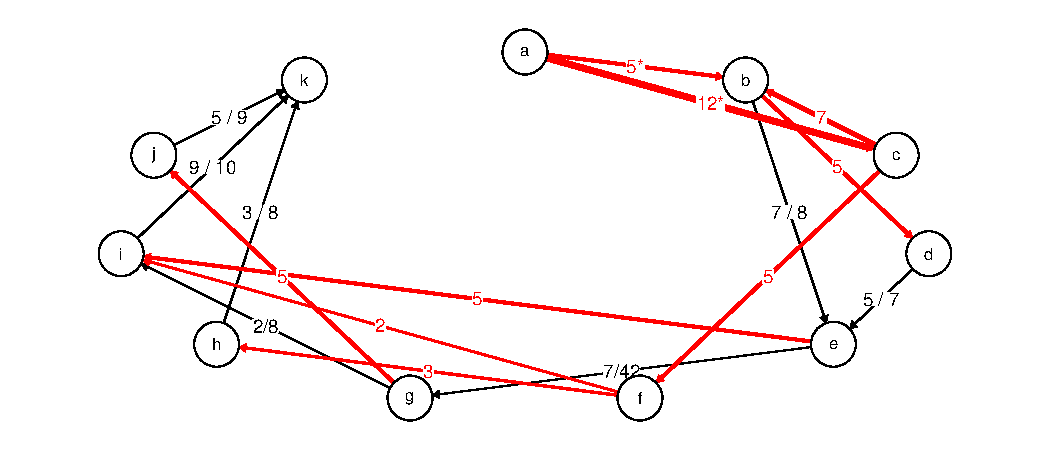
\includegraphics[width=\maxwidth]{figure/unnamed-chunk-2} 

}



\end{knitrout}


    The mean of this distribution is simply the inverse rate, while the median is the mean times $\ln 2$, and the mode
    is zero.

    \[
        \begin{aligned}
            \text{Mean } &= \lambda^{-1}\\
            \text{Median } &= \lambda^{-1} \cdot \ln(2)\\
            \text{Mode } &= 0
        \end{aligned}
    \]

    @ With probability $0.7$, the toss of an Olympic shot putter travels $D = 60 + X$ meters, where $X$ is an
    exponential random variable with expected value $\lambda = 10$. Otherwise, with probability $0.3$, a foul is
    committed by stepping outside of the shotput circle and we say $D = 0$. Find and graph the cumulative distribution
    of random variable $D$. (Note: This is an example of a random variable with a mixed discrete-continuous
    distribution.)
    @@ This is another case of a random variable transformation. We know $X$ has exponential distribution with
    $\lambda=10$, and that $D = 60 + X$. Let's establish this first.

    \[
        \begin{aligned}
            X = 10 e^{-10x} && D = 60 + X\\
            P\left( 60 + X \le d\right) &\Rightarrow& P \left( X \le d - 60 \right)\\
            &\Rightarrow& D = 10 e^{-10(d - 60)}
        \end{aligned}
    \]

    Now that we've determined $D$ we can take a look at the rest of the statement regarding foul rate. Let $Z$ be the
    random variable denoting success (S) or failure (F). We know that $P(Z=S) = 0.7$ and conversely $P(Z=F)=0.3$, so now
    let's transform our transformed $D$.

    \[
        \begin{aligned}
            D = 10 e^{-10(d - 60)} && Z = 0.7 D\\
            P(Z = S) &\Rightarrow& P(0.7D = S)\\
            P\left(D = \frac{S}{0.7} \right)  &\Rightarrow& P(0.7D = S)\\
            &\Rightarrow& 14.2857 \exp\left(-10 \left( \frac{s}{0.7} - 60 \right)\right)
        \end{aligned}
    \]

\begin{knitrout}
\definecolor{shadecolor}{rgb}{0.969, 0.969, 0.969}\color{fgcolor}

{\centering 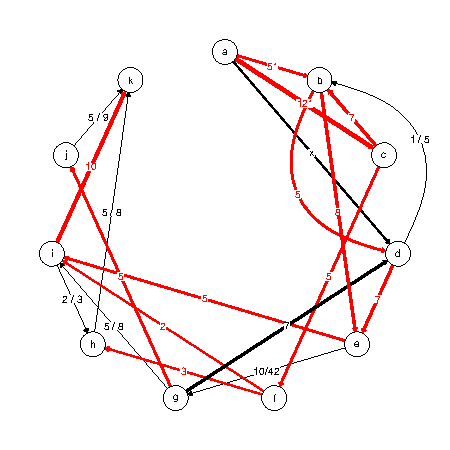
\includegraphics[width=\maxwidth]{figure/unnamed-chunk-3} 

}



\end{knitrout}


    As you can see, having only 70\% succeed radically shifts the distribution, and would be much better to be
    eliminated if examining the average throw.

\end{easylist}

\end{document}
